% Section 1: Trench Warfare in WWI
%---------------------------------------------------------------------------

\begin{frame}{Trench Warfare in WWI}
  \begin{itemize}
    \item On the Western Front, 
    early advances ground to a halt and stagnated into trench warfare
    \item Technologies like artillery and machine guns made the war one of the bloodiest in human history
  \end{itemize}
\end{frame}

\begin{frame}{Trench Warfare in WWI}
  \begin{center}
  \includegraphics[width=1\textwidth]{figures/fig131.png}
  \end{center}
  What's the \textbf{NE}?
\end{frame}

\begin{frame}{Unexpected Truces Emerge}
  Christmas Day Truce, 1914:
  \begin{center}
    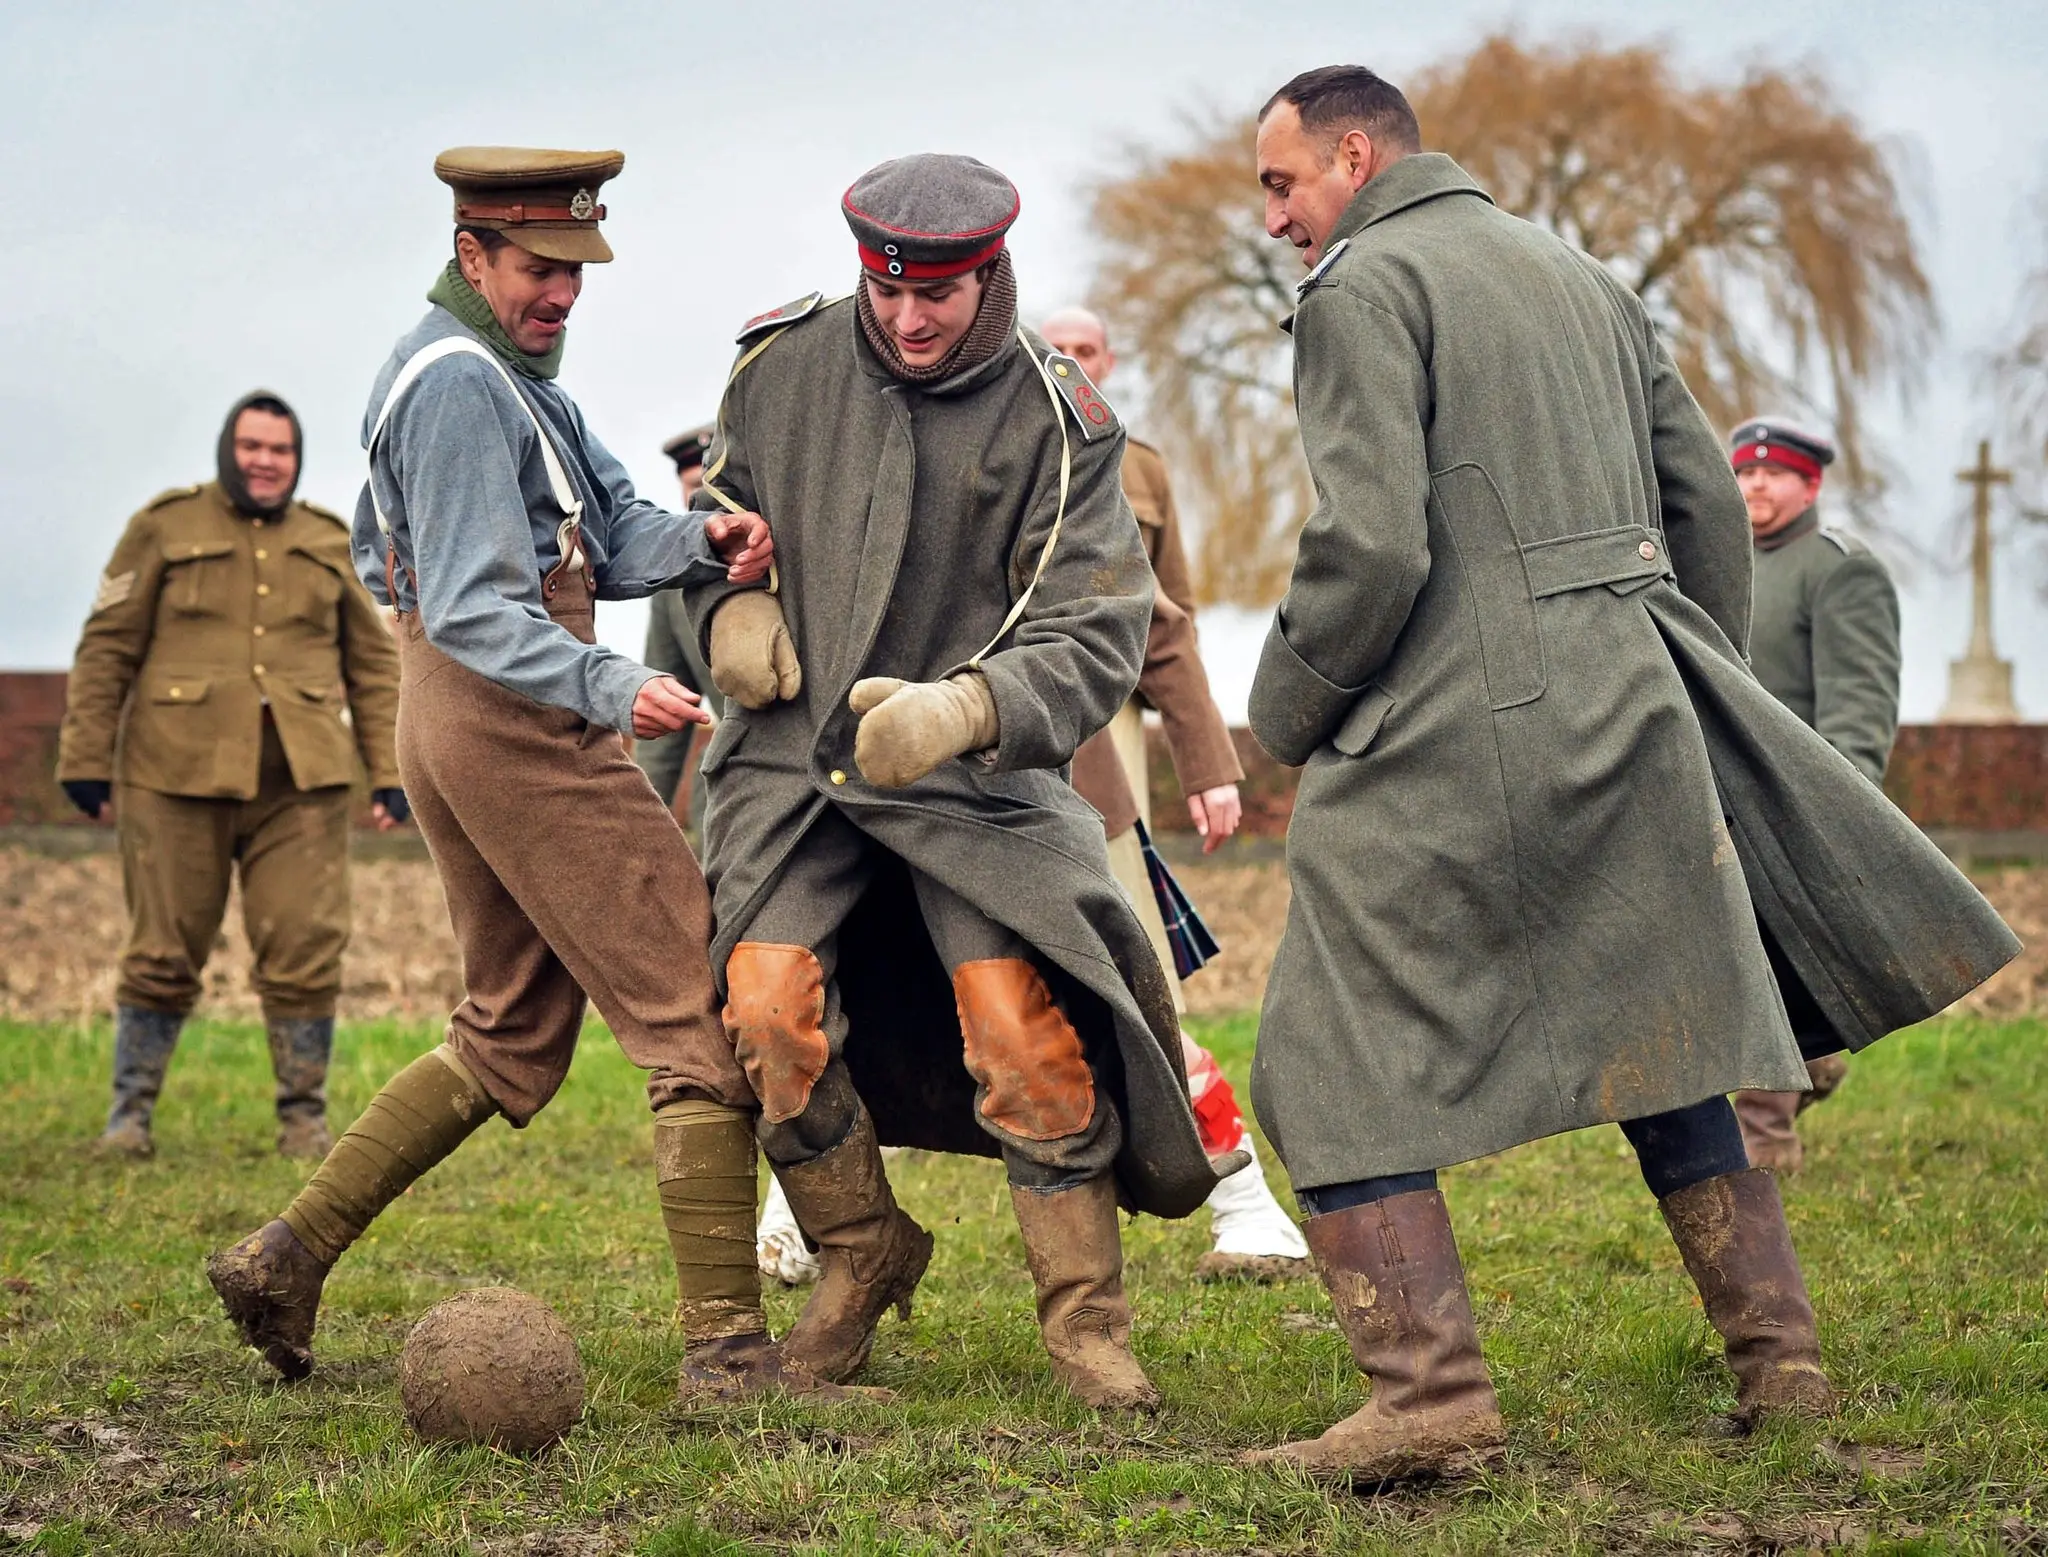
\includegraphics[width=.75\textwidth]{figures/hughes24-superJumbo.png} 
  \end{center}
  {\footnotesize Image Credit: Stephanie Lecocq/European Pressphoto Agency}
\end{frame}

\begin{frame}{Unexpected Truces Emerge}
  \begin{quote}
    \footnotesize 

    So regular were [the Germans] in their choice of targets, times of shooting, and number of rounds fired, that, after being in the line one or two days, Colonel Jones had discovered their system, and knew to a minute where the next shell would fall. His calculations were very accurate, and he was able to take what seemed to uninitiated Staff Officers big risks, knowing that the shelling would stop before he reached the place being shelled.

    I was having tea with A Company when we heard a lot of shouting and went out to investigate. We found our men and the Germans standing on their respective parapets. Suddenly a salvo arrived but did no damage. Naturally both sides got down and our men started swearing at the Germans, when all at once a brave German got on to his parapet and shouted out “We are very sorry about that; we hope no one was hurt. It is not our fault, it is that damned Prussian artillery.”
  \end{quote} 
\end{frame}

\begin{frame}{The puzzle of trench truces}
  \begin{itemize}
    \item How did cooperation between enemy armies achieved and sustained?
    \item One answer might be that in these parts of the front, interactions were \textbf{repeated} between the same units
  \end{itemize} 
\end{frame}

\begin{frame}{Constructing a Repeated Game}
  \begin{itemize}
    \item Suppose that Allied and German forces anticipate that they will play this game $T$ times 
  \end{itemize}
  \begin{center}
    \includegraphics[width=.5\textwidth]{figures/fig131.png}  
  \end{center}
  \begin{itemize}
    \item A \textit{strategy} will be made up of $T$ \textit{actions}; 
    one for each time this stage game is played
  \end{itemize}
\end{frame}

% \begin{frame}{Constructing a Repeated Game}
%   To represent this as an extensive form tree, lets suppose that $T=2$:
%   \begin{itemize}
%     \item If neither side sees what their opponent's strategy was yesterday, each player has 3 info sets
%     \item So each side has eight possible strategies:
%     \begin{itemize}
%       \item (\textit{Kill$_1$}, \textit{Kill$_2$} if \textit{Kill$_1$} or \textit{Miss$_1$})
%       \item (\textit{Kill$_1$}, \textit{Kill$_2$} if \textit{Kill$_1$} else \textit{Miss$_2$} if \textit{Miss$_1$})
%       \item (\textit{Kill$_1$}, \textit{Miss$_2$} if \textit{Kill$_1$} else \textit{Kill$_2$} if \textit{Miss$_1$})
%       \item (\textit{Kill$_1$}, \textit{Miss$_2$} if \textit{Kill$_1$} or \textit{Miss$_1$})
%       \item ...
%     \end{itemize}
%   \end{itemize}
% \end{frame}

% \begin{frame}{Constructing a Repeated Game}
%   \begin{center}
%     \includegraphics[width=1\textwidth]{figures/fig132.png} 
%   \end{center} 
% \end{frame}

\begin{frame}{Constructing a Repeated Game}
  To represent this as an extensive form tree, lets suppose that $T=2$:
  and suppose that the history of all past plays are \textbf{common knowledge} 
  \begin{itemize}
    \item each player will have five info sets; one for day 1, and four in day 2 
    \item What does the extensive form game look like?
  \end{itemize}
\end{frame}

\begin{frame}{Constructing a Repeated Game}
  \begin{center}
    \includegraphics[width=1\textwidth]{figures/fig133.png} 
  \end{center} 
\end{frame}

\begin{frame}{Constructing a Repeated Game}
  Let's generalize what a strategy in \textit{any} \alert{finitely repeated game} with \alert{common knowledge} will look like:
  \begin{itemize}
    \item If a game has $T$ periods, and each player has $m$ actions at each stage,
    \item there is one initial info set, $m^2$ info sets in period 2, $m^4$ info sets in period 3, ..., $m^{2(T-1)}$ in the last period 
    \item A complete strategy is made up of $1 + m^2 + m^4 + ... + m^{2(T-1)}$ actions 
  \end{itemize}
  In an \alert{infinitely repeated game}, there will be an infinite number of actions in each strategy
\end{frame}

\begin{frame}{Constructing a Repeated Game}
  How to model streams payoffs over time?
  \begin{itemize}
    \item We could just add up all of the per-stage payoffs across an entire history
    \item But for infinitely-long histories, this sum would blow up and not make much sense
    \item Instead, we will use \alert{present value} calculations
  \end{itemize}
\end{frame}

\begin{frame}{Present Values}
  Suppose that I have an income stream where I earn $w_t$ dollars in every year $t$
  \begin{itemize}
    \item Suppose that there is a single \alert{discount factor} $\delta$ which captures how much I value income tomorrow compared to income today
    \item My present value over my whole income stream is 
    $$ w_1 + \delta w_2 + \delta^2 w_3 + \delta^3 w_4 + ... + \delta^{T-1} w_T $$
    \item It makes sense to assume that $0<\delta<1$ because I should probably care about tomorrow to some extent, but not as much as today
  \end{itemize}
\end{frame}

\begin{frame}{Present Values}
  What about calculating a present value of an \alert{infinte stream} of payoffs?
  \begin{itemize}
    \item It turns out:  
    $$ x + \delta x + \delta^2 x + \delta^3 x + ... + \delta^{\infty} x $$
    \item actually converges to $\frac{x}{1-\delta}$ as long as $\delta<1$ 
  \end{itemize}
\end{frame}

\begin{frame}{Check Your Understanding}
  Suppose you are deciding between three different payoff streams:
  \vspace{5mm}

  \begin{center}
  \begin{tabular}{|c|c|c|c|}
    \textbf{Period} & \textbf{Stream A} & \textbf{Stream B} & \textbf{Stream C} \\ \hline 
    1 & 15 & 25 &  5 \\ 
    2 & 15 & 15 & 10 \\ 
    3 & 15 & 10 & 20 \\ 
    4 & 15 &  5 & 30 \\
  \end{tabular}
  \end{center}

  \vspace{5mm}
  Which has the \textbf{highest present value} when $\delta =0.8$?
  \pause
  
  Stream A: 44.28, \textbf{Stream B: 45.9}, Stream C: 41.16
\end{frame}

\begin{frame}{Going back to the trenches}
  \begin{center}
    \includegraphics[width=.8\textwidth]{figures/fig133.png} 
  \end{center}  
  This was our extensive form game for only 2 periods
\end{frame}

\begin{frame}{Going back to the trenches}
  Now suppose that we have a potentially very large $T$

  How can we find a SPNE?

\end{frame}

\begin{frame}{Going back to the trenches}
  Suppose that we are already at the last period $T$ of the $T$-period trench warfare game 

  Suppose that the Allies total payoff stream value so far is $A^{T-1}$ and the Germans is $G^{T-1}$ 
  \begin{center}
    \includegraphics[width=.7\textwidth]{figures/tab137.png} 
  \end{center}
  What will happen?
  \pause

  \begin{itemize}
      \item Allies will Shoot to \textbf{Kill},
      Germans will Shoot to \textbf{Kill}
  \end{itemize}
\end{frame}

\begin{frame}{Going back to the trenches}
  Now that we know the $T$ stage will end in $(Kill, ~Kill)$, we can look one period back to what will happen in $T-1$: 
  \begin{center}
    \includegraphics[width=.7\textwidth]{figures/fig138.png}
  \end{center}
  What will happen?
  \pause
  \begin{itemize}
      \item Both will shoot to \textbf{Kill} in $T-1$, knowing they will both shoot to kill in $T$
  \end{itemize}
\end{frame}

\begin{frame}{Trench Game with Finite stages}
  By now, you should get the idea:
  \begin{block}{Insight}
    If the stage game has a unique NE, then any finitely repeated version will have a unique SPNE which is just the repetition of the single-stage NE. No cooperation is sustainable 
  \end{block}

  So what was going on with those spontaneous truces?
\end{frame}

\begin{frame}{Infinitely Repeated Trench Game}
  \begin{itemize}
    \item The problem with that last equilibrium we found was that you have to know \textit{exactly when the game will end} to use backwards induction 
    \item But for World War I infantrymen, they didn't know how long it would be until the fronts shifted or their division was rotated out
    \item We will have to extend our models to allow for \alert{indefinite horizons}
  \end{itemize} 
\end{frame}

\begin{frame}{Infinitely Repeated Games}
  Suppose the probability that at each stage, with probability $p$, the game continues and with $(1-p)$, the game ends and you get $u=0$

  The \textbf{expected present value} of a stream of payoffs $u_1, u_2, ...$ is then:
  $$ V = u_1 + p d u_2 + p^2 d^2 u_3 + ... = \sum_{t=1}^{\infty}(pd)^{t-1}u_t $$
\end{frame}

\begin{frame}{Infinitely Repeated Games}
  Now if we let $\delta = pd$ represent the discount factor from both time preferences and the likelihood of the game terminating:
  $$ V = \sum_{t=1}^{\infty}(pd)^{t-1}u_t = \sum_{t=1}^{\infty}\delta^{t-1}u_t $$

  Which is exactly the same as the expected present value of a stream of \textbf{infinite} payments
\end{frame}

\begin{frame}{SPNE in Repeated Games}
  A strategy profile is SPNE if and only if in each period and for each history, the prescribed action is optimal given:
  \begin{itemize}
    \item the other players act according to their strategies in the current period
    \item all players act according to their strategies in all future periods
  \end{itemize}
\end{frame}

\begin{frame}{Grim Trigger in the Trench Game}
  Consider the following strategy: 
  \begin{itemize}
    \item In period 1, choose miss
    \item In period $t>1$, choose miss if both chose miss in all past periods, else choose kill
  \end{itemize}
  This type of strategy is known as \alert{Grim Trigger} because this type of player starts out cooperative, but if wronged once, they will always shoot to kill
\end{frame}
